\begin{minipage}{0.55\textwidth}
    \begin{figure}[h]
    \centering
    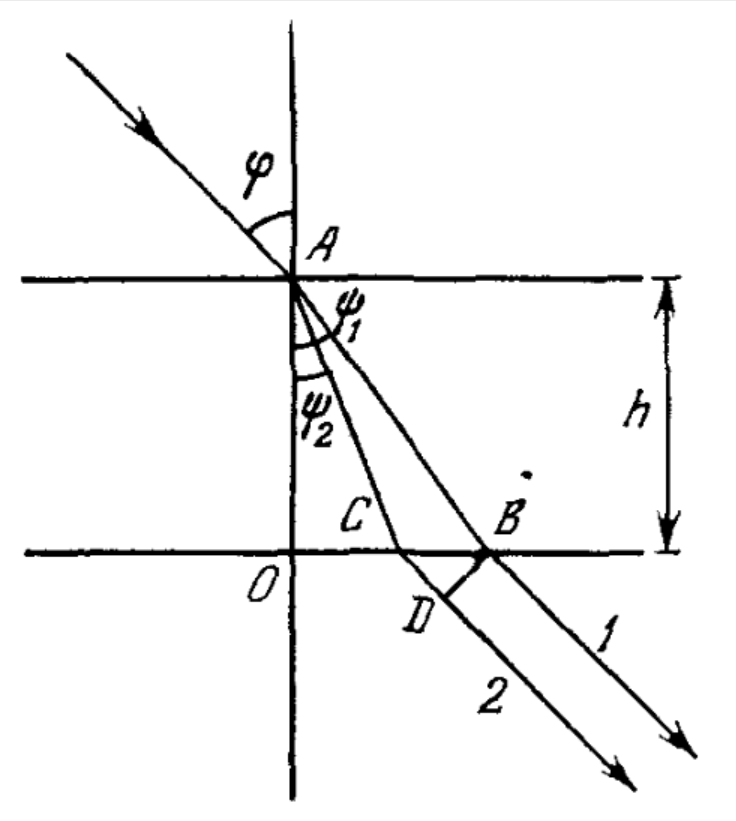
\includegraphics[width=0.7\textwidth]{images/intercolor.png}
    \caption{The setup to get an inreferencion of polarized light that is similar to what we had.}
    %\label{fig:}
\end{figure}
\end{minipage}
\hfill
\begin{minipage}{0.35\textwidth}
    We obtain that the key role plays the wavelength of the light
    \begin{equation*}
        \Delta \varphi = 2 \pi \frac{\Delta}{\lambda}.
    \end{equation*}
    So we will differ the plates (K) regarding to relation of its $\Delta$ to $\lambda$.
\end{minipage}
